\documentclass[22pt]{beamer}
% \documentclass[handout]{beamer}
% add theme and color theme https://www.overleaf.com/learn/latex/Beamer#Reference_guide
\setbeamertemplate{navigation symbols}{arguments} % hides navigation buttons
\setbeamertemplate{footline}[frame number]
\usepackage[utf8]{inputenc}
\usepackage{minted}
\usepackage{graphicx}
\usepackage{comment}
%% \usepackage[b]{beamer}
\usemintedstyle{tango}
\pagenumbering{roman}

\title{Docker something}
\author{Julia Winkler}
\date{19.06.2024}

\begin{document}
\maketitle

\begin{frame}{Gliederung}
    \tableofcontents
\end{frame}


\begin{frame}[t]
    \frametitle{Wiso, Weshalb, Warum?}
    \begin{itemize}
        \item hier motivation und coole usecases
        \item independant entwicklungs umgebung \pause
        \item Kubernetes \pause
        \item ...
    \end{itemize}
\end{frame}

\begin{frame}[t]
    \frametitle{Wer ist Moby Dock?}
    \begin{itemize}
        \item 1
    \end{itemize} 
    %% TODO: bild vom docker wahl
\end{frame}

\begin{frame}[t]
    \frametitle{Was ist Docker?}
    \begin{itemize}
        \item 1
    \end{itemize} 
    %% bild
\end{frame}

\begin{frame}[t]
    \frametitle{Wichtige Begriffe}
    Docker
    Container
    Image
    Dockerfile
    Docker Compose
    Docker Hub
    Docker Desktop
\end{frame}

\begin{frame}[t]
    \frametitle{Hello World}
    \begin{itemize}
        \item Wechsel zu cmd
        \item docker --help
        \item docker run hello-world
        \item docker run --help
    \end{itemize} 
    %% docker run mit versch Argumenten
\end{frame}

\begin{frame}[t]
    \frametitle{Basic commands}
    \begin{itemize}
        \item docker run
        \item docker ps / docker ps -a
        \item 
    \end{itemize} 
\end{frame}

\begin{frame}[t]
    \frametitle{Dockerfile}
    \begin{itemize}
        \item FROM, CMD \& Entrypoint, RUN, COPY, ARG
        \item Layer
    \end{itemize} 
    %% docker build
\end{frame}

\begin{frame}[t]
    \frametitle{Dockerfile}
    \begin{figure}[h]
        \centering
        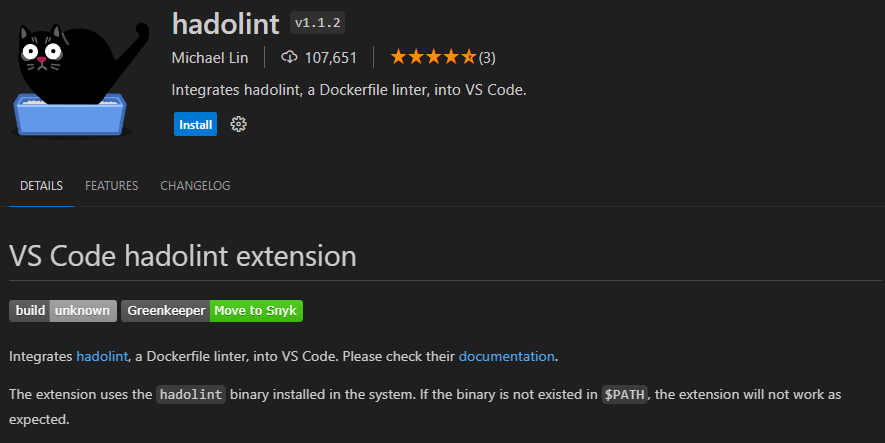
\includegraphics[width=0.5\textwidth]{Hadolint.png}
        \caption{}
    \end{figure}
\end{frame}


%% vllt Docker mit ubuntu for exec, it, start, stop, name

\begin{frame}[fragile]
    \frametitle{Python bsp}
    \inputminted[fontsize=\footnotesize, frame=lines]{dockerfile}{../examples/Dockerfile.cmd}
    %% run mit volume und port
    %% start, stop, rm
\end{frame}

\begin{frame}[t]
    \frametitle{Volumes}
    \begin{itemize}
        \item 
    \end{itemize} 
\end{frame}

\begin{frame}[fragile]
    \frametitle{React}
    \inputminted[fontsize=\footnotesize, frame=lines]{dockerfile}{../examples/Dockerfile.cmd}
\end{frame}

\begin{frame}[t]
    \frametitle{Multistage builds}
    \begin{itemize}
        \item 1
    \end{itemize} 
\end{frame}

\begin{frame}[fragile]
    \frametitle{React - Multistage}
    \inputminted[fontsize=\footnotesize, frame=lines]{dockerfile}{../examples/Dockerfile.cmd}
\end{frame}

\begin{frame}[t]
    \frametitle{Dockerfile Best practices}
    \begin{itemize}
        \item RUN commands
        \item Order of COPY
        \item Volumes
        \item Multistage
    \end{itemize} 
\end{frame}

\begin{frame}[t]
    \frametitle{Docker Compose}
    \begin{itemize}
        \item Vorteile
        \item UseCases
    \end{itemize} 
\end{frame}

\begin{frame}[fragile]
    \frametitle{Docker Compose zu Python}
    \inputminted[fontsize=\footnotesize, frame=lines]{dockerfile}{../examples/Dockerfile.cmd}
\end{frame}

\begin{frame}[fragile]
    \frametitle{Docker Compose Webapp}
    \inputminted[fontsize=\footnotesize, frame=lines]{dockerfile}{../examples/Dockerfile.cmd}
\end{frame}

\begin{frame}[t]
    \frametitle{important Commands}
    \begin{itemize}
        \item docker run
        \item docker build
        \item docker push, pull
        \item docker ps -a
        \item docker rm / rmi
        \item ...
    \end{itemize} 
\end{frame}

\begin{frame}[t]
    \frametitle{Coole Quellen und so weiter}
    \begin{itemize}
        \item 1
    \end{itemize} 
\end{frame}

\begin{comment}

\begin{frame}[t]
    \frametitle{title}
    \begin{itemize}
        \item 1
    \end{itemize} 
\end{frame}

\begin{frame}[fragile]
    \frametitle{title}
    \inputminted[fontsize=\footnotesize, frame=lines]{dockerfile}{../examples/Dockerfile.cmd}
\end{frame}

\begin{wrapfigure}{l}{0.25\textwidth}
    \centering
    \includegraphics[width=0.25\textwidth]{contour}
\end{wrapfigure}

\begin{figure}[h]
\centering
\includegraphics[width=0.5\textwidth]{spiral}
\caption{}
\end{figure}
    
\end{comment}

\end{document}